\documentclass{jfm}

% Compilation
\usepackage{silence} % Silence latex compiler warnings
\WarningFilter{latex}{Command \@xhline has changed} % Filter out warning
  % caused by redefinition between jfm.cls class and array (loaded by
  % siunitx)

% Import custom style file containing common packages and options
\setlength{\paperheight}{\pdfpageheight} % JFM class removes paperheight definition and hyperref raises a warning

% Import custom style file containing common packages and options
\usepackage{preamble}
\graphicspath{{./Figures/}}

% Discrete Fourier Transform
\newcommand{\GenP}{\hat{P}_m}
\newcommand{\POne}{\hat{P}_1}
\newcommand{\PTwo}{\hat{P}_2}
\newcommand{\PThree}{\hat{P}_3}
\newcommand{\PFour}{\hat{P}_4}

% Continuous Fourier Transform
\newcommand{\GenPk}{\hat{P} (\kappa)}
\newcommand{\PZerok}{\hat{P} (0)}

% Define custom math symbols
\DeclareMathOperator{\cn}{Cn}
\DeclareMathOperator{\sgn}{sgn}
\DeclareMathOperator{\Ur}{Ur}
\DeclareMathOperator{\Sk}{Sk}
\DeclareMathOperator{\As}{As}
%\DeclareMathOperator{\Bi}{Bi}

\newcommand{\hilbert}{\mathcal{H}}

% Define custom math functions
\DeclarePairedDelimiter{\round}{\lfloor}{\rceil}

% Define \im as Roman i
\newcommand{\im}{\mathrm{i}}
% Replace epsilon with varepsilon
\renewcommand*{\epsilon}{\varepsilon}

%% Use \thalf and \squart commands from JFM class
%\newcommand\squart{\ensuremath{{\textstyle\frac{1}{4}}}}
%\newcommand\thalf{\ensuremath{{\textstyle\frac{1}{2}}}}

\linenumbers{}

\title{Wind-Induced Changes to Surface Gravity Wave Shape in Shallow Water}

\author{Thomas J. Zdyrski \and Falk Feddersen}

\begin{document}

\maketitle

\begin{abstract}
Wave shape (\eg{} wave skewness and asymmetry) impacts sediment
transport, remote sensing, and ship safety.
Previous work by the authors showed that wind (via changes in surface
pressure) affects wave shape in intermediate and deep water.
This effect was most pronounced as the depth decreased.
Here, this work investigates the interaction of wind and wave shape in
shallow water.
A multiple-scales analysis of long waves propagating over a shallow,
flat bottom and forced by a Jeffreys-type surface pressure produces a
Korteweg-de Vries (KdV)-Burgers governing the wave profile.
The evolution of an initially symmetric solitary wave is calculated
numerically.
The wave's height, skewness, and asymmetry are investigated as functions
of time and pressure magnitude.
The setup's parameters are grouped to form invariant scalings,
providing a simple means of translating between different parameter
ranges.
These results are in qualitative agreement with prior results in
intermediate and deep water.
\end{abstract}

\section{Introduction}

The study of wind's interaction with ocean waves has a long history, beginning
with \citet{jeffreys1925formation} and continuing to be an active field
of
research~\citep[\eg][]{janssen1991quasi,donelan2004limiting,sulivan2010dynamics}.
Early
theories~\citep[\eg][]{jeffreys1925formation,miles1957generation,phillips1957generation}
were primarily interested in calculating wind-induced growth rates
and often employed a phase-averaging technique.
However, it is also known that wind can influence wave
shape~\citep[\eg][]{leykin1995asymmetry,feddersen2005wind,zdyrski2020wind},
which can be represented by third-order shape statistics such as
skewness and asymmetry, corresponding to the wave's vertical and
horizontal asymmetry, respectively.
Wave shape influences sediment transport
\citep[\eg][]{drake2001discrete, gonzalez2007seabed} which modulates
beach morphodynamics~\citep[\eg][]{hoefel2003wave}.
Additionally, wave skewness affects the returned signal in radar
altimetry~\citep[\eg][]{hayne1980radar,huang1983non},
and wave asymmetry influences ship response to wave
impacts~\citep[\eg][]{soares2008abnormal,oberhagemann2013prediction}.
Therefore, understanding how wind influences these shape statistics is a
matter of practical importance.

When the water depth $h$ is small compared to the wavelength $\lambda$,
waves are classified as shallow-water waves $kh \ll 1$ (with $k
\coloneqq 2 \pi/\lambda$).
Waves in shallow water differ qualitatively from those in intermediate
to deep water where $kh \sim 1$ or $\gg 1$, respectively.
For waves with amplitudes $a_0$ much less than the water depth $h$,
leveraging the small parameter $a_0/h$ yields the Boussinesq equations
for waves in small waves in shallow water.
The waves' interactions with the bottom modifies the dispersion
relation, causes shallow-water wave trains to be weakly dispersive, and
permits a special class of waves wherein dispersion balances nonlinear
focusing known as solitary waves.
These have appeared in environments ranging from nonlinear optical pulses
\citep[\eg][]{kivshar1993dark} to astrophysical dusty plasmas
\citep[\eg][]{sahu2012nonextensive}.
One of the simplest models for solitons is the Korteweg-de Vries (KdV)
equation, which incorporates dispersion and nonlinearity.
When augmented with a dissipative term, this becomes the KdV-Burgers
equation.
The KdV-Burgers appears across disciplines including damped internal
tides \citep[\eg][]{sandstrom1995dissipation}, electron waves in
graphene \citep[\eg][]{zdyrski2019effects}, and viscous flow in blood
vessels \citep[\eg][]{antar1999weakly}.
In order to investigate the interaction of wind and surface waves in
shallow water, we introduce a wind-induced pressure term in the
Boussinesq equations in \cref{sec:derivation}.
This will produce a KdV-Burgers equation governing the surface profile's
evolution, which we will solve numerically.
We analyze the wave height, skewness, and asymmetry in
\cref{sec:results}.
Finally, we discuss wind speeds and compare the results to intermediate
and deep-water waves in \cref{sec:discussion}.

\section{\label{sec:derivation} Derivation of KdV-Burgers Equation}
We begin by specifying the assumptions and governing equations; we will
then derive the KdV-Burgers equation and clarify the numerical scheme.

\subsection{Governing Equations}
We will treat the flow as irrotational and inviscid throughout the
fluid and neglect surface tension by restricting to wavelengths $\lambda
\gg \SI{2}{\centi\meter}$.
Furthermore, we restrict to planar wave propagation in the $+x$
direction.
Finally, we choose a coordinate system with $z=0$ at the mean water level and
a horizontal, flat bottom located at $z=-h$.
Then, the incompressibility condition and standard boundary conditions
are%
\footnote{
  We used the gauge freedom to absorb the Bernoulli ``constant'' $C(t)$
  in the dynamic boundary condition into the definition of $\phi$.
}
\begin{alignat}{2}
  0 &= \phi_{xx} + \phi_{zz} &&\qq{on}
  -h < z < \eta \,, \label{eq:laplace}\\
  0 &= \phi_{z} &&\qq{on} z=-h \,, \label{eq:bottom_bc}\\
  \phi_{z} &= \eta_{t} + \phi_{x} \eta_{x} &&\qq{on} z = \eta \,,
  \label{eq:kinematic_bc}\\
  \qq*{and} 0 &= \frac{p}{\rho_w} + g\eta + \phi_{t} +
  \frac{1}{2} \bqty{\phi_{x}^2 + \phi_{z}^2} &&\qq{on} z=
  \eta \,. \label{eq:dynamic_bc}
\end{alignat}
Here, $\eta(x,t)$ is the wave profile, $\phi(x,z,t)$ is the velocity
potential $\vec{u} = \grad{\phi}$, $p(x,t)$ is the surface pressure,
$g$ is the acceleration due to gravity, and $\rho_w$ is the water
density.
We are seeking a solitary, progressive wave with properties
\begin{gather}
  \eta(\vec{x},t) \to 0 \qq{and} \pdv{\eta(\vec{x},t)}{x} \to 0 \qq{as}
  \abs{\vec{x}} \to \infty \,,
\end{gather}
with similar conditions on $\vec{u}$.
We are parameterizing our initial wave by four dimensional quantities:
the mean depth, bottom horizontal velocity, wave height, and wavelength.
We will choose a coordinate system where the average bottom horizontal
velocity vanishes:
\begin{equation}
  \overline{ \pdv{\phi}{x} } = 0 \qq{on} z=-h \,,
  \label{eq:bot_bc_horz}
\end{equation}
with the overline an average over a wavelength.
Additionally, we assume the surface pressure $p(x,t)$ is a Jeffreys-type
forcing \citep{jeffreys1925formation}:
\begin{equation}
  p(x,t) = P \pdv{\eta(x,t)}{x} \,.
\end{equation}
Here, $P$ is proportional to $(U-c)^2$, with $U$ the wind speed and $c$
the wave speed (\cf{} \cref{sec:press_mag}), and $P>0$ corresponding to
wind in the same direction as the wave.
We use a Jeffreys forcing for its analytic simplicity and clear
demonstration of wind-wave coupling.
Though Jeffrey's separated sheltering mechanism is likely only relevant
in special situations (\eg{} near breaking
\citealp{banner1976separation} or for steep waves under strong winds
\citealp{tian2013evolution,touboul2006interaction}),
a fully dynamic coupling between wind and waves---necessary for an
accurate surface pressure---is outside the scope of this paper.

\subsection{\label{sec:nondim} Nondimensionalization}
We will nondimensionalize with the known characteristic scales: the
horizontal length scale $L$ over which $\eta$ changes
rapidly, expressed as an effective wavenumber $k_E \coloneqq 2 \pi/L$;
the (initial) wave amplitude $a_0 = H_0/2$ (\ie{} half the wave height
$H_0$); the depth $h$; the gravitational acceleration $g$; and the wind
speed $U$ expressed as a pressure magnitude $P \propto \rho_a (U-c)^2$.
Denoting nondimensional variables with an prime, we have
\begin{equation*}
  \begin{aligned}
  x &= \frac{x'}{k_E} = h \frac{x'}{\sqrt{\mu_E}}\,, \\
  z &= h z' \,,
  \end{aligned}
  \qquad
  \begin{aligned}
  t &= \frac{t'}{k_E\sqrt{g h}}
    = \frac{t'}{\sqrt{\mu_E}} \sqrt{\frac{h}{g}} \,, \\
  P &= \epsilon P' \frac{\rho_w g}{k_E}
    = \frac{\epsilon}{\sqrt{\mu_E}} P' \rho_w g h \,,
  \end{aligned}
  \qquad
  \begin{aligned}
  \eta &= a_0 \eta' = h \epsilon \eta' \,, \\
  \phi &= \phi'\frac{a_0}{k_E}\sqrt{\frac{g}{h}}
    = \frac{\phi'\epsilon}{\sqrt{\mu_E}}\sqrt{g h^3} \,.
  \end{aligned}
\end{equation*}
We have defined the parameters $\epsilon a_0/2h$ and $\mu_E \coloneqq
(kh)^2$ and chosen $\order{P k_E/(\rho_w g)} = \order{\epsilon}$.
These three small, nondimensional parameters define our system.
We will later require $\order{\epsilon} = \order{\mu_E}$.
Now, our nondimensional equations take the form
\begin{alignat}{2}
  0 &= \mu_E \phi'_{x'x'} + \phi'_{z'z'} &&\qq{on}
    -1 < z' < \epsilon \eta' \,, \label{eq:laplace_nondim} \\
  0 &= \phi'_{z'} &&\qq{on} z'=-1 \,, \label{eq:bottom_bc_nondim} \\
  \phi'_{z'} &= \mu_E \eta'_{t'} +
    \epsilon \mu_E \phi'_{x'} \eta'_{x'} &&\qq{on} z' = \epsilon \eta' \,,
    \label{eq:kinematic_bc_nondim} \\
  0 &= \epsilon P' \eta'_{x'} +  \eta' + \phi'_{t'} + \frac{1}{2}
    \pqty{\epsilon \phi_{x'}^{\prime \, 2} + \frac{\epsilon}{\mu_E}
    \phi_{z'}^{\prime \, 2}} &&\qq{on} z'= \epsilon \eta' \,.
    \label{eq:dynamic_bc_nondim}
\end{alignat}
Note that this is equivalent to choosing a set of units wherein $h = g =
\rho_w = 1$.
We will drop the primes henceforth for readability.

\subsection{Depth Dependence of \texorpdfstring{$\phi$}{Velocity Potential}}
Here, we modify the Bousinesq equation's derivation provided by
\citet{mei2005nonlinear} to include a surface pressure forcing.
Laplace's equation \cref{eq:laplace_nondim} and the bottom boundary
condition \cref{eq:bottom_bc_nondim} determine the depth dependence of
$\phi$ by expanding about $z=-1$:
\begin{equation}
  \phi(x,y,z,t) = \sum_{n=0}^\infty (z+1)^n\phi_n(x,y,t) \,.
\end{equation}
A standard calculation \citep[\eg][]{mei2005nonlinear} yields an
expansion of $\phi$ in terms of $\mu_E \ll 1$:
\begin{equation}
  \phi = \phi_0 - \frac{1}{2}\mu_E (z+1)^2\partial^2_x\phi_0 +
  \frac{\mu_E^2}{24}(z+1)^4\partial^4_x\phi_0 +
  \order{\mu_E^3} \,.
\end{equation}
For convenience, we define $\varphi \coloneqq \phi_0$.
Substituting this expansion into the two remaining boundary equations,
\cref{eq:kinematic_bc_nondim,eq:dynamic_bc_nondim}, and recalling that
they are evaluated at $z=\epsilon \eta$, we have reduced our system to
the Boussinesq equations with a pressure forcing term,
\begin{gather}
  \partial_t \eta + \partial_x^2 \varphi + \epsilon \partial_x
    \pqty{\eta \partial_x \varphi} -\frac{1}{6}\mu_E \partial^4_x
    \varphi = \order{\mu_E^2} \label{eq:kinematic_bc_varphi} \,, \\
  \partial_t \varphi + \epsilon P \partial_x \eta + \eta -
    \frac{1}{2}\mu_E \partial_t \partial_x^2 \varphi +
    \frac{1}{2}\epsilon\pqty{\partial_x \varphi}^2 = \order{\mu_E^2} \,.
    \label{eq:dynamic_bc_varphi}
\end{gather}
Further, we will now assume $\order{\epsilon} = \order{\mu_E} \ll 1$.

\subsection{\label{sec:shallow_water} Perturbation Expansion}
We expand the time $t$ in terms of multiple timescales $t_n =
\epsilon^n t$ for $n= 0,1$, so all time derivatives become $\partial_t \to
\partial_{t_0} + \epsilon \partial_{t_1}$.
Then, we write $\eta$ and $\varphi$ in asymptotic series of $\epsilon$,
\begin{equation}
  \eta(x,t) = \sum_{k=0}^{\infty} \epsilon^k
    \eta_{k+1}(x,t_0,t_1) \qq{and}
  \varphi(x,t) = \sum_{k=0}^{\infty} \epsilon^k
    \varphi_{k+1}(x,t_0,t_1,) \,.
\end{equation}

Now, we will reduce the Bousinessq equations
\cref{eq:kinematic_bc_varphi,eq:dynamic_bc_varphi} to the KdV equations
following a similar method to \citet{mei2005nonlinear}.
\subsection{Shallow Water Wave Equations}
Collecting order-one terms $\order{\epsilon^0}$ from
\cref{eq:kinematic_bc_varphi,eq:dynamic_bc_varphi} gives
\begin{equation}
  \pdv{\eta_0}{t_0} + \pdv[2]{\varphi_0}{x} = 0 \qq{and}
  \eta_0 + \pdv{\varphi_0}{t_0} = 0 \,.
\end{equation}
These shallow-water wave equations have left- and right-moving wave
solutions.
Restricting to right-moving waves gives $\varphi_0 = f_0(x-t_0,t_1)$ and
$\eta_0 = f'_0(x-t_0,1)$, with $f_0' \coloneqq \eval{\partial_{\theta}
f_0(\theta,t_1)}_{\theta = x-t_0}$.
We have restricted to right-moving waves and neglected the $x$-linear
term in $\varphi_0$ since we chose $u = \partial_x \varphi = 0$ at the
bottom~\cref{eq:bot_bc_horz}.

\subsection{\label{sec:int_first_order} KdV Burgers Equation}
Continuing to the next order of perturbation theory, we retain terms of
order $\order{\epsilon}$:
\begin{gather}
    \pdv{\eta_1}{t_0} + \pdv[2]{\varphi_{1}}{x} =
      -\pdv{\eta_0}{t_1} - \pdv{x} \pqty{\eta_0 \pdv{\varphi_0}{x}} +
      \frac{1}{6} \frac{\mu_E}{\epsilon} \pdv[4]{\varphi_0}{x}
  \\
    \eta_1 + \pdv{\varphi_1}{t_0} = -P \pdv{\eta_0}{x} -\pdv{\varphi_0}{t_1}
      + \frac{1}{2} \frac{\mu_E}{\epsilon} \frac{\partial^3 \varphi_0}
        {\partial t_0 \partial^2 x}
      - \frac{1}{2} \pqty{ \pdv{\varphi_0}{x} }^2
  \,.
\end{gather}
Inserting our leading order solutions for $\eta_0$ and $\varphi_0$ while
eliminating $\eta_1$ gives
\begin{equation}
  \pqty{\pdv[2]{x} - \pdv[2]{t_0}} \varphi_1 = -2 \pdv{f_0'}{t_1} +
    P\pdv{\eta_0}{t_0}{x} - 3 f_0' f_0'' - \frac{1}{3} \frac{\mu_E}{\epsilon}
    f_0^{(4)} \,.
\end{equation}
The homogeneous equation is again the shallow-water wave equation for
$\varphi_1$.
Since the right-hand side is a resonant forcing, it must vanish.
Thus, converting back to $\eta_0$ gives
\begin{equation}
  \pdv{\eta_0}{t_1} + \frac{3}{2}
    \eta_0 \pdv{\eta_0}{x} + \frac{1}{6} \frac{\mu_E}{\epsilon}
    \pdv[3]{\eta_0}{x} = -P \frac{1}{2} \pdv[2]{\eta_0}{x} \,.
  \label{eq:kdv_burgers}
\end{equation}
This is the Korteweg-de Vries (KdV)-Burgers equation.
Note that the pressure term, $P \partial^2_x \eta_0$, can act as either
a positive viscosity for offshore, damping wind or a negative viscosity
when onshore wind causes wave growth.
As written, \cref{eq:kdv_burgers} has a rescaling symmetry where $\mu_E
\to \lambda^2 \mu_E$ is equivalent to taking $(x,t_0,t_1,P) \to
(x,t_0,t_1,P)/\lambda$.
Therefore, we now fix the length scale (equivalently, $k_E$) by choosing
$\mu_E = 6 \epsilon$.
The KdV-Burgers equation is not known to have any closed form solutions,
so we will instead solve this numerically.

\subsection{Initial Conditions}
For an initial condition, we use the solitary wave solutions of
the unforced KdV equation, \ie{} \cref{eq:kdv_burgers} with $P=0$.
For better numerical accuracy, we also boost into a frame moving with
the unforced solitary wave speed by including a term $U\partial_x
\eta_0$ on the left-hand side of \cref{eq:kdv_burgers}.
Using the solution from \citet{dingemans1997water} (as quoted in
\citealp{brun2018convective}) the solitary wave solution to the KdV
equation is
\begin{equation}
  \eta_0 = H_0 \sech^2\pqty{\frac{x - c_1 t_1}{\Delta}}
  \qq{with}
  \Delta = \sqrt{\frac{8}{H_0}}
  \qq{and}
  c_1 = U + \frac{H_0}{2} \,.
\end{equation}
$H_0>0$ is an order-1 parameter.
We set $U=-H_0/2$ so the unforced wave is stationary.
Reverting back to dimensional variables (with primes denoting
dimensionless), we now choose $H_0'=2$ so that $a_0$ is half the maximum
of $\eta_0$.
The solitary wave solution of the unforced KdV equation balances
dispersion $\partial_x \eta_0$ with focusing nonlinearity $\eta_0
\partial_x \eta_0$; the introduction of a dissipative term $P
\partial_x^2 \eta_0$ will disrupt the balance and cause shape changes.

\subsection{Numerics}
We will solve \cref{eq:kdv_burgers} numerically.
The spatial domain has periodic boundary conditions and $N_x = 400$
points spread over a domain of length $L' = 20$.
This yields a spacing $\Delta x' = 0.05$, with $x' = 0, \Delta x',
2\Delta x', \ldots L' - \Delta x'$.
The simulation runs from $t'= 0$ to $T' = 3$, inclusive, with
$N_t = \num{4.8e5}$ points, yielding a spacing $\Delta t' = T'/(N_t-1)
\approx \num{6.25e-6}$.
We found that slowly ramping $P'$ up from $0$ at $t'=0$ to its full
value did not qualitatively modify the results, so we do not utilize
such a ramp-up here.

The PDE \cref{eq:kdv_burgers} is discretized in space using a
second-order central finite difference method and in space using a
\nth{3}-order Runge-Kutta scheme.
For numerical stability, we must also include a hyperviscosity term
$-\nu_{\text{bi}} \partial_x^4$ on the right-hand side of
\cref{eq:kdv_burgers},
\begin{equation}
  \pdv{\eta'_0}{t'_1} - \pdv{\eta'_0}{x'} + \frac{3}{2}
  \eta'_0 \pdv{\eta'_0}{x'} + \pdv[3]{\eta'_0}{{x'}} =
  -P \frac{1}{2} \pdv[2]{\eta'_0}{{x'}} - \nu_{\text{bi}}
  \pdv[4]{\eta'_0}{{x'}} \,,
  \label{eq:kdvb_nondim}
\end{equation}
with $\nu_{\text{bi}} = \num{3e-3}$, which we solve with the initial
condition
\begin{equation}
  \eta'_0(x',t_1=0) = 2 \sech^2\pqty{\frac{x'}{2}} \,.
  \label{eq:initial_condition}
\end{equation}

We will quantify the wave shape according to the wave height $H$,
\begin{equation}
  H = \max(\eta) - \min(\eta) \,,
  \label{eq:height_def}
\end{equation}
as well as the skewness $\Sk$ and $\As$,
\begin{equation}
  \Sk \coloneqq \frac{\langle \eta^3 \rangle}{\langle \eta^2
  \rangle^{3/2}} \
  \qq{and}
  \As \coloneqq \frac{\langle \hilbert \Bqty{\eta^3} \rangle}{\langle
    \eta^2 \rangle^{3/2}} \,.
  \label{eq:shape_stats_def}
\end{equation}
Here, we have used the wave average
\begin{equation}
  \langle f \rangle \coloneqq \frac{1}{L'} \int_{-L'/2}^{L'/2} f
  \dd{x} \,,
\end{equation}
and $\hilbert$ is the Hilbert transform.
Since these definitions carry a factor of the domain size $\sqrt{L'}$,
we will normalize the skewness $\Sk$ by the initial skewness $\Sk_0$.

\section{\label{sec:results} Results}
Given the one free parameter $P k_E/(\rho_w g \epsilon)$ of the
KdV-Burgers equation \cref{eq:kdvb_nondim}, we can now plot the results
for different pressure magnitudes $P k_E/(\rho_w g \epsilon)$.
We are particularly interested in the differences between onshore wind
($P > 0$) and offshore wind ($P < 0$).

\begin{figure}
  \centering
  { % Put \phantomsubcaption in their own group to prevent it from
    % affecting the main figure's numbering
    \phantomsubcaption{}\label{fig:snapshots_solitary:a}
    \phantomsubcaption{}\label{fig:snapshots_solitary:b}
  }
  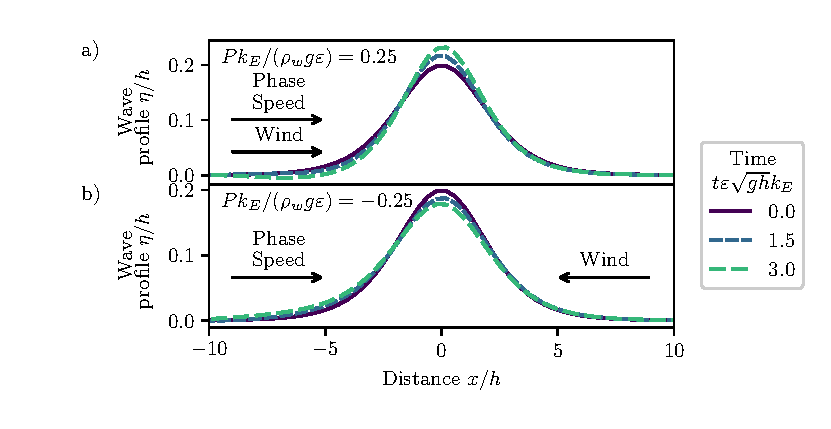
\includegraphics{Snapshots-Positive-Negative-Production.eps}
  \caption{
    Evolution of a solitary wave profile under
    \subref{fig:snapshots_solitary:a}
    onshore and
    \subref{fig:snapshots_solitary:b}
    offshore Jeffreys forcing.
    The nondimensional wave height $\eta/h$ is plotted for
    nondimensional distance $-10 \le x/h \le 10$.
    Results are shown for $\epsilon=0.1$, $\mu_E = 0.6$, and $\abs{P
    k_E/(\rho_w g \epsilon)} = 0.25$ nondimensional slow times $t
    \epsilon \sqrt{gh} k_E = 0$, $1.5$, and $3$, as indicated in the
    legend.
    The arrows denote the direction of wave propagation (phase speed) or
    wind direction.
  }\label{fig:snapshots_solitary}
\end{figure}

The snapshots of the wave profile $\eta/h$ in
\cref{fig:snapshots_solitary} qualitatively show how the wave shape
evolves over nondimensional time $t \epsilon \sqrt{g h} k_E$ when
plotted against the nondimensional distance $x/h$.
The onshore wind (\cref{fig:snapshots_solitary:a}, $Pk_E/(\rho_w g
\epsilon) = 0.25$) increases the slope of the wave with time, while the
offshore wind (\cref{fig:snapshots_solitary:b}, $Pk_E/(\rho_w g
\epsilon) = -0.25$) decreases it.
However, the windward side of the wave always becomes steeper than the
leeward side (up to \SI{8}{\percent} steeper for the time period shown).
Thus, despite the waves starting from symmetric, solitary-wave initial
conditions, the wind induces a horizontal asymmetry in the wave slope.
This asymmetry is also apparent in the wave profile itself, particularly
on the rear face ($x<0$) of the wave.
Namely, the offshore wind (\cref{fig:snapshots_solitary:b}) raises the
rear base of the wave (near $x/h = -5$) relative to its initial profile
(purple line).
Conversely, an onshore wind (\cref{fig:snapshots_solitary:a}) depresses
the rear face, even forming a small depression below the still water
level near $x/h = -6$ at $t\epsilon \sqrt{gh} k_E=3$ (green line).

\begin{figure}
  \centering
  { % Put \phantomsubcaption in their own group to prevent it from
    % affecting the main figure's numbering
    \phantomsubcaption{}\label{fig:statistics_solitary:a}
    \phantomsubcaption{}\label{fig:statistics_solitary:b}
    \phantomsubcaption{}\label{fig:statistics_solitary:c}
  }
  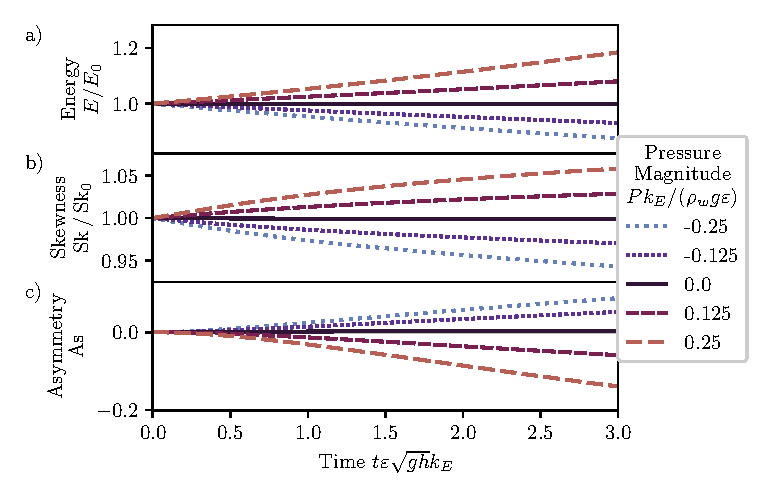
\includegraphics{Skew-Asymm-Production.eps}
  \caption{
    Shape statistics of a solitary profile under onshore and offshore
    Jeffreys forcing are shown for nondimensional slow time $t \epsilon
    \sqrt{gh} k_E = \numrange{0}{3}$.
    The
    \subref{fig:statistics_solitary:a}
    height,
    \subref{fig:statistics_solitary:b}
    skewness normalized by the initial time, and
    \subref{fig:statistics_solitary:c}
    asymmetry are defined in
    \cref{eq:height_def,eq:shape_stats_def}.
    Results are shown for $\epsilon=0.1$, $\mu_E = 0.6$, and $P
    k_E/(\rho_w g \epsilon) = 0$, $\pm 0.125$, and $\pm 0.25$, as
    indicated in the legend.
    The solid black line corresponds to the unforced case, $P = 0$, and
    shows no growth or asymmetry and a constant, positive skewness.
  }\label{fig:statistics_solitary}
\end{figure}

To quantify the effect of wind on wave shape,
\cref{fig:statistics_solitary} shows shape statistics as functions of
the nondimensional slow time $t \epsilon \sqrt{g h} k_E$ for onshore
wind ($P k_E/(\rho_w g \epsilon) = 0.125$ and $0.25$), offshore wind ($P
k_E/(\rho_w g \epsilon) = -0.125$ and $-0.25$), and the unforced case
($P k_E/(\rho_w g \epsilon) = 0$).
We plot all cases for initial steepness $\epsilon = 0.1$ up to slow
time $t'_1 = 3$, corresponding to $3/\epsilon = 30$ wave periods.
The height (\cref{fig:statistics_solitary:a}) begins at $H_0/h = 2
\epsilon = 0.2$ and shows the onshore wind ($P>0$) causing wave
accelerating wave growth while the offshore wind ($P<0$) causes decay
which slows over time.
We can even see this qualitatively in the accelerating crest growth
(\cref{fig:snapshots_solitary:a}) and decelerating crest decay
(\cref{fig:snapshots_solitary:b}) of \cref{fig:snapshots_solitary} at
$x=0$.

We can also quantify wave shape by the third-order moments, skewness
(\cref{fig:statistics_solitary:b}) and asymmetry
(\cref{fig:statistics_solitary:c}).
The onshore (offshore) causes the wave to become more (less) skewed over
time.
The skewness is nearly symmetric with respect to $\pm P$ about one.
The initial profile has zero asymmetry, and the unforced case
$P=0$ maintains zero asymmetry over time.
However, the onshore wind causes a backwards tilt and negative
asymmetry, while the offshore wind increases the asymmetry causing the
wave to tilt forwards, as seen in \cref{fig:snapshots_solitary}.
Notice that $\abs{\As}$ is larger for onshore winds than offshore winds.
The definitions of the skewness and asymmetry are insensitive to scaling
of the waveform $\eta \to \lambda \eta$, so this effect is not simply
caused by the wave's growth under an onshore wind.
Instead, over \SI{80}{\percent} of the discrepancy between the $P>0$ and
$P<0$ asymmetries (\cref{fig:statistics_solitary:c}) arises from the
rear half of the wave.
This is consistent with the observation from
\cref{fig:snapshots_solitary} that the rear side has a much more
apparent shape change, and we will discuss the cause
\cref{sec:physical_reason}.
Though this analysis focuses on solitary waves, we also investigated the
effect of wind on periodic waves using the cnoidal-wave KdV solutions as
initial conditions.
The pressure induced shape statistics were qualitatively similar to
those derived for solitary waves, so they are not shown here for
brevity.

\section{\label{sec:discussion} Discussion}

\subsection{\label{sec:press_mag} Wind Speed Estimation}
In \cref{sec:nondim}, we chose to nondimensionalize the pressure as $P
k_E/(\rho_w g) = \order{\epsilon}$.
Now, we estimate the wind speed associated with such a pressure
to show that this choice is reasonable.
First we need the growth rate of the energy $E$, which we numerically fit
to
\begin{equation}
  E \coloneqq \rho_w g \int_{-\infty}^{\infty} {\eta'}_0^2 \dd{x}
  \propto \frac{1}{1 - \gamma' t'}
  \qq{with}
  \gamma' \coloneqq b \bqty{\frac{P k_E}{\rho_w g}}
  \,,
  \label{eq:actual_energy}
\end{equation}
and $b = 1.992 \pm \num{1e-4}$.
This is close to the analytic approximation for the decay rate $\gamma'
= (4/15) (P k_E/\rho_w g)$ derived, for example, with a secondary
multiple scales approximation of the KdV-Burgers equation acting on a
solitary wave in eq.\ 72 of \citealp{zdyrski2019effects} (with
$\mathcal{A}=1$, $\mathcal{B} = 3/2$, $\mathcal{C} = 1$, $\mathcal{G} =
(P k_E)/(2 \rho_w g)$, and $c_0 = H_0 = 2$).
This is consistent with the observation in
\cref{fig:snapshots_solitary,fig:statistics_solitary} that the energy
(and height) change accelerates for $P>0$ but decelerates for $P<0$.
Alternatively, we can approximate the energy growth rate from the
KdV-Burgers equation \cref{eq:kdvb_nondim} with the standard procedure
\citep[\eg][]{mei2005nonlinear} of multiplying by $\eta'_0$ and
integrating from $x'=-\infty$ to $\infty$:
\begin{equation}
  \pdv{t'_1} \int_{-\infty}^{\infty} {\eta'}_0^2 \dd{x}
  = \int_{-\infty}^{\infty} P' \pqty{\pdv{\eta'_0}{x'}}^2
  \dd{x} \,.
\end{equation}
The left integral is the energy \cref{eq:actual_energy}, so
redimensionalizing gives the energy growth rate $\gamma$,
\begin{equation}
  \frac{\gamma}{c k_E} \coloneqq
  \frac{1}{c k_E E} \pdv{E}{t}
  = \frac{P k_E}{\rho_w g} \frac{\langle (\partial_x \eta)^2 \rangle}
    {\langle (k_E \eta)^2 \rangle}
  = \frac{1}{5} \frac{P k_E}{\rho_w g}
  \,,
  \label{eq:gamma_vs_P_solitary}
\end{equation}
with the phase speed $c = \sqrt{gh}$.
In the final equation, we evaluated the growth rate for the initial
solitary wave profile \cref{eq:initial_condition}.
Note that this is consistent with the growth rate found in
\cref{eq:actual_energy} for small times $\gamma t \ll 1$.

Additionally, \citet{jeffreys1925formation} theory relates this growth
rate to the wind speed $U_z$ (the subscript giving the measurement
height $z$) as
\begin{equation}
  \frac{\gamma}{\omega} = S_z \frac{\rho_a}{\rho_w}
    \pqty{\frac{U_z}{c}-1} \abs{\frac{U_z}{c}-1} \,,
  \label{eq:gamma_vs_u_jeffreys}
\end{equation}
with $S_z$ a sheltering parameter potentially dependent on the
$\epsilon$, $\mu_E$, and $U_z/c$.
Combining this with \cref{eq:gamma_vs_P_solitary} gives
\begin{equation}
  U_z = c \pqty{1 \pm \sqrt{\frac{1}{5} \abs{\frac{P k_E}{\rho_w g}}
    \frac{\rho_w}{\rho_a} \frac{1}{S_z}}} \,.
  \label{eq:U_vs_P}
\end{equation}
Here, the $\pm$ corresponds to onshore ($+$) or offshore ($-$) winds.
Note that changing the wind direction (\ie{} sign of $Pk_E/(\rho_w g)$,
or $\pm$ sign) while holding the surface pressure magnitude
$\abs{Pk_E/(\rho_w g)}$ constant means $\abs{U_z}$ onshore will be
larger than $\abs{U_z}$ offshore.

\Citet{donelan2006wave} provides a parameterization for shallow-water
waves that depends on airflow separation: $S_{\lambda/2} =
\epsilon \sqrt{\mu} \bqty{4.91-3.98 H\Bqty{\epsilon \sqrt{\mu}
\bqty{(U_{\lambda/2}/c)^2-1} - 1}}$, with $H$ the Heaviside function,
$U_z$ measured at $z=\lambda/2$, and $\mu \coloneqq (kh)^2$.
We can evaluate \cref{eq:U_vs_P} for the parameters used in
\cref{sec:results} ($\epsilon=0.1$, $\mu_E = 0.6$, $Pk/(\rho_w g
\epsilon) = 0.25$). This yields a non-separated flow,
$\epsilon \sqrt{\mu} \bqty{(U_{\lambda/2}/c)^2-1} < 1$.
While \citet{donelan2006wave} measured this parameterization for
periodic waves, we will assume it holds approximately for solitary waves
and take $\lambda = 2 \pi/k_E = \SI{20}{\meter}$, corresponding to a
depth of $h = \SI{2.5}{\meter}$ and initial wave height $H_0 =
\SI{0.5}{\meter}$.
Then, this gives the wind speed at $z=\SI{10}{\meter}$ as $U_{10} =
\SI{21}{\meter\per\second}$, a reasonable wind speed for strongly forced
shallow-water waves.

\subsection{\label{sec:physical_reason} Physical Interpretation}
In \cref{sec:results}, we noted that the rear face of the waves in
\cref{fig:snapshots_solitary} showed marked shape differences between
onshore and offshore wind, while the front faces were rather similar.
We can understand this by considering the fluid velocity in this
co-moving frame.
The surface pressure $p \propto \partial_x \eta$ only does work
close to the wave where $\partial_x \eta$ is significant.
The water reaching the front face has only been acted upon by pressure
for a short distance, so the work done by the wind is minimal and causes
little shape change.
Once the water reaches the rear face, the surface pressure has acted
over a longer distance, performed more work, and yielded a larger shape
change.
Onshore wind (\cref{fig:snapshots_solitary:a}) does positive work---see
the increasing wave height in \cref{fig:statistics_solitary:a}.
This additional kinetic energy causes the downward-moving water to
overshoot $z=0$ at the rear base of the wave, leading to the depression
seen in \cref{fig:snapshots_solitary:a}.
Conversely, offshore wind does negative work and the decreased kinetic
energy delays the flow's return to the still water level in
\cref{fig:snapshots_solitary:b}.
As discussed in \cref{sec:results}, this discrepancy between the front
and rear wave faces is responsible for much of the variation between
onshore asymmetry and offshore asymmetry in
\cref{fig:statistics_solitary:c}.

\subsection{Comparison to Intermediate and Deep Water}
Here, we have coupled wind to waves in shallow water.
A previous study \citep{zdyrski2020wind} instead coupled wind and waves
in intermediate to deep water.
That study investigated the effect of wind on Stokes-like waves as
solitary waves are not possible.
However, qualitative agreement is still found between these two studies.
\Cref{fig:statistics_solitary} shows that, for a fixed time $t \neq 0$,
the asymmetry increases as the pressure $P$ increases.
\Figname{} 4(a) of \citet{zdyrski2020wind} displayed a similar trend for
the corresponding Jeffreys pressure profile with positive (negative)
pressure increasing (decreasing) the asymmetry.
In addition to the Jeffreys-type forcing employed here,
\citet{zdyrski2020wind} also utilized a Generalized Miles (GM)-type
wherein the pressure was proportional to $\eta$ shifted by a distance
parameter $\psi_P/k$.
However, results for GM forcings were not included here since the GM
forcing gives rise to a nonlocal KdV equation and produces unphysical
effects such as the growth of higher harmonics under offshore winds.
Finally, the lack of shallow water wind and wave-shape experiments
precludes a comparison to experimental data as in
\citet{zdyrski2020wind}.
While we are unable to directly compare the effects of wind on
shallow-water solitary waves with those on deep-water Stokes-like waves,
we do have qualitative agreement between these two regimes.

\section{Conclusion}
Prior results~\citep{zdyrski2020wind} in intermediate and deep water
demonstrated that wind, acting though an $\eta$-dependent surface
pressure, can generate shape changes that become more pronounced in
shallow water.
This motivated the current work which used a multiple scales analysis to
couple weak wind with mild-slope long waves, \ie{} $H_0/h \sim (k_E h)^2
\sim P k/(\rho_w g) \ll 1$.
This derivation produced a KdV-Burgers equation governing the wave
profile $\eta$.
We utilized a symmetric solitary wave satisfying the unforced KdV
equation as our initial condition.
A third-order Runge Kutta solver determined the time-evolution of the
surface profile, and we extracted height, skewness, and asymmetry as
functions of time and pressure magnitude.
For onshore wind (positive $P$), wave height and skewness increased with
time while asymmetry decreased, with offshore wind producing opposite
effects.
Furthermore, these effects were enhance for strong pressures, reducing
to the unforced case for $P=0$.
The shape statistics found here show qualitative agreement with the
results in intermediate and deep water, and future work on periodic
shallow-water waves would allow a direct, quantitative comparison with
the periodic deep-water waves.
Declaration of Interests. The authors report no conflict of interest.

\appendix

% Bibliography
\bibliographystyle{jfm}
\bibliography{references}

\end{document}
